\chapter{The Tokai-to-Kamioka experiment}
\label{chp:t2kdetector}

The Tokai-to-Kamioka (T2K) experiment is a long baseline neutrino oscillation experiment based in Japan and its purpose is to study neutrino oscillations: specifically a precision measurement of the neutrino oscillation parameters $\Delta m_{23}^{2}$ and $\sin ^{2} \theta_{23}$ and to increase the measurement to the leptonic CP violating phase $\delta_{CP}$, which are mentioned in Chapter 1. The experiment produces a beam of intense muon neutrinos at J-PARC (Japan Proton Accelerator Research Complex) in Tokai, which is located on the far east coast of Japan in Ibaraki Prefecture. The muon neutrino beam travels 295 km west towards the far detector Super-Kamiokande (see Chapter 3.)  These neutrinos are detected by other detectors such as ND280 and INGRID, before they oscillate and reach Super-Kamiokande which is important with regards to measuring the neutrino oscillation parameters. ND280 and Super-Kamiokande are off-axis detectors, meaning that they are placed 2.5$\degree$ off axis to the centre of the neutrino beam - this allows for the peak of the energy of the muon neutrinos to be at 0.6 GeV, meaning that the neutrino oscillation on the 295 km baseline is maximised, and the reduced spread in muon neutrino energy means that these detectors are far less susceptible to potential backgrounds. This chapter explains production of the muon neutrino beam from the JPARC proton beam line and the near detector complex.

\subsection{Neutrino beam production}

\subsubsection{JPARC proton beam production}

The production of a proton beam from JPARC is due to three accelerators, the LINAC (linear accelerator), an RCS (rapid cyclic synchrotron) and the main ring synchrotron (MR). A negative hydrogen ion is accelerated to a kinetic energy of 400 MeV, from which a beam of protons is created by converting the negative hydrogen ion beam using charge-stripping foils. This proton beam is then accelerated to a kinetic energy of 3 GeV by the RCS, and about 5\% of the bunches produced from this process are passed to the MR where the proton beam will be accelerated up to 30 GeV. 

\subsubsection{Neutrino beam production}

The neutrino beam is produced using a primary and a secondary beamline as shown in Figure \ref{fig:nubeamline}. The primary beamline involves taking the proton beam from the MR and targeting it towards the direction of Kamioka and then transferring it through a succession of beam monitors which measure facets of the neutrino beam including the beam profile, intensity and position. The beam monitor which is closest to the graphite target measures the "Protons-On-Target" (POT), a value used to determine the neutrino beam flux. The secondary beamline involves taking the proton bunches and passing them through a target station, the decay volume and the beam dump. After interacting with the target station, the proton bunches are collimated through a 1.7 m graphite rod where the collimated hole the proton bunches pass through are 30 mm in diameter. Beam profile reconstruction occurs in the OTR (Optical Transition Radiation) monitor, made up of titanium alloy foil placed at a 45 degree angle in order to intercept the beam. As the proton beam enters the foil, the visible light that is produced escapes through a collection of mirrors and is then captured by a charge injection device camera, which creates the beam profile. After beam profiling, the proton beam then impacts upon a graphite rod target which is 91.4 cm long and 2.6 cm in diameter - this collision produces secondary hadrons, including pions which are focused by three magnetic horns. These magnetic horns can be used to produce either a muon neutrino or muon antineutrino beam depending on the polarity of the 250kA current they are pulsed with. If a +250 kA current is used, the positive pions and kaons produced can go on to make muon neutrino beams wheareas if a -250 kA current is used negative pions and kaons can decay to create muon antineutrino beams (both are shown in Equation \ref{eq:nubeam}). The +250 kA mode is called Forward Horn Current (FHC) mode and the -250 kA mode is called Reversed Horn Current (RHC) mode, and the analysis in this thesis will occur in FHC mode only. 

\begin{equation}
\begin{array}{lll}
\pi^{+} & \longrightarrow \mu^{+}+\nu_{\mu} & \text { FHC } \\
\pi^{-} & \longrightarrow \mu^{-}+\overline{\nu_{\mu}} & \text { RHC }
\end{array}
\label{eq:nubeam}
\end{equation}

A 75 ton volume beam dump made of graphite and iron stops the particles, specifically the protons, secondary hadrons and mesons which have a momentum below 5 GeV/c end up being absorbed by the beam dump. A muon monitor is placed after the beam dump in order to directly measure the the beam intensity and beam direction - muons can be used to monitor the beam properties because along with the neutrinos these are the main particles produced from the pion decay. After the muon monitor, a nucleon emulsion plate detector measures the flux and momentum of the muons. 

\subsection{Near detectors}

\subsubsection{ND280}

ND280 is a near detector which sits 280 m from the graphite target. It is an off-axis detector, meaning that just like Super-Kamiokande, it is placed 2.5 $\degree$ off-axis from the center of the beam. This stems from the relationship between the energy of the neutrinos produced from the decay of the pions, a relationship shown in Equation \ref{eq:piondecay}. 

\begin{equation}
    E_{\nu}=\frac{m_{\pi}^{2}-m_{\mu}^{2}}{2\left(E_{\pi}-\sqrt{E_{\pi}^{2}-m_{\pi}^{2}} \cos \theta\right)}
\label{eq:piondecay}
\end{equation}

where $E_{\pi}$ is the energy of the parent pion and $\theta$ is the scattering angle between the direction of the outgoing neutrino and the direction of the parent pion's momentum. $m_{pi}$ is the parent pion mass and $m_{\mu}$ is the mass of the outgoing muon. Figure \ref{fig:energyangle} shows the neutrino energy from pion decay plotted against the energy of the parent pion for a range of off-axis angles. 

\begin{figure}
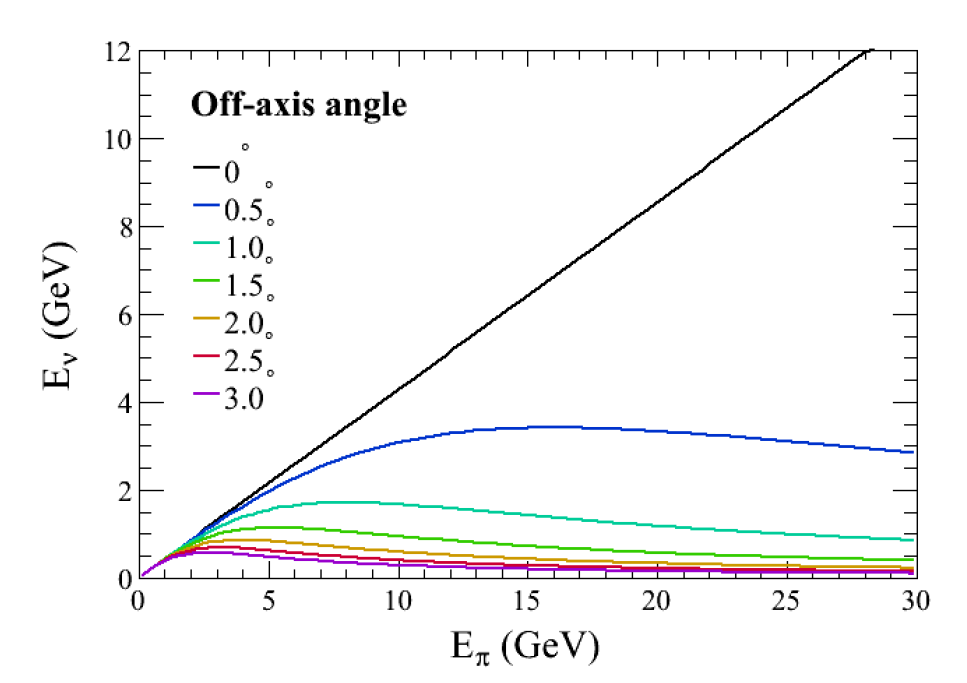
\includegraphics[width=\textwidth]{Figures/energyangle.png}
\caption{Energy of the neutrino plotted against the energy of the parent pion for multiple different off-axis angles}
    \label{fig:energyangle}
\end{figure}

As off-axis angle increases, the intensity of the neutrino beam decreases, and therefore picking an off-axis angle of 2.5 $\degree$ at which to place the ND280 detector complex strikes a good balance between keeping a high beam intensity while ensuring a peak energy of 0.6 GeV in order to have the neutrino oscillation be maximised at 295km. The relationship between muon neutrino oscillation probability and muon neutrino energy is shown at the top in Figure \ref{fig:nuprobosc}, and at the bottom the muon neutrino flux 295 km away from the graphite target can be seen for three different off-axis angles.

\begin{figure}
    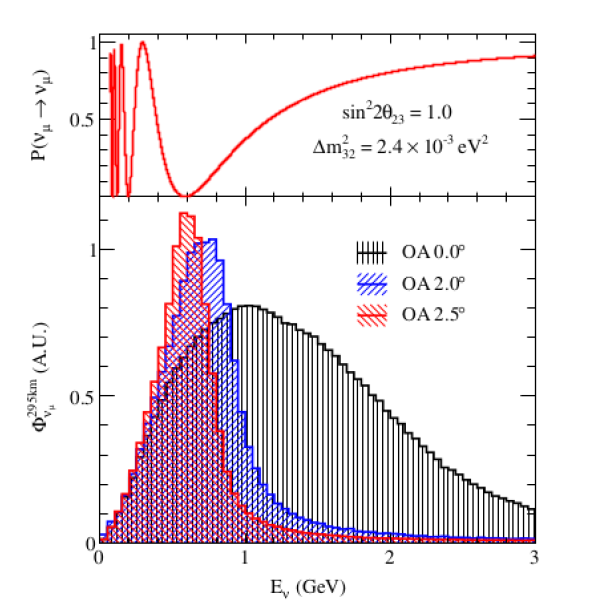
\includegraphics[width=\textwidth]{Figures/nuprobosc.png}
    \caption{The probability of survival of muon neutrinos (top plot) and neutrino beam flux at the 295km far detector (bottom) Taken from \cite{t2kcollaborationT2KNeutrinoFlux2013}.}
    \label{fig:nuprobosc}
\end{figure}

Figure \ref{fig:ND280_schematic} shows a schematic of the ND280 detector complex. It has three main goals: firstly, to measure the cross sections of muon neutrino interactions, so neutrino-nucleus interaction models can reduce their systematic uncertainties. Secondly, measuring the component of the neutrino beam which is made of electron neutrinos, hence being able to better constrain the background to electron neutrino appearance at the far detector. And thirdly, to determine the event rate at Super-Kamiokande by measuring the energy spectrum of the muon neutrinos produced. 

\begin{figure}
    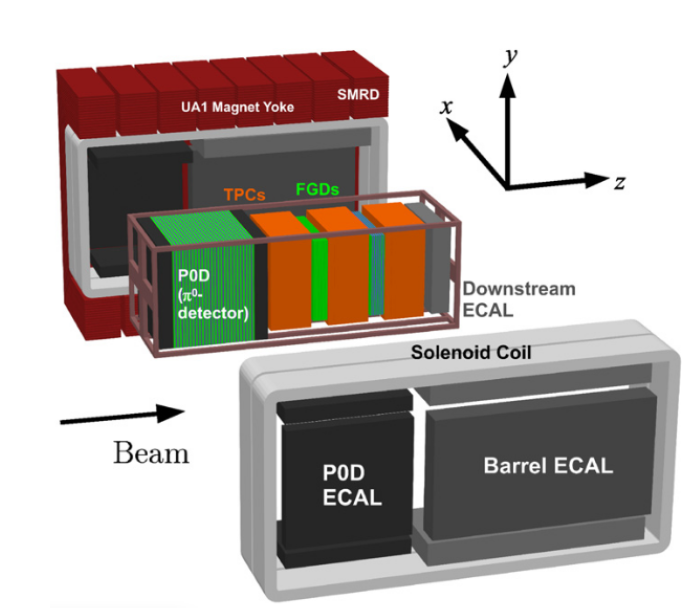
\includegraphics[width=\textwidth]{Figures/nd280_complex.png}
    \caption{Near detector ND280 schematic taken from \cite{t2kcollaborationT2KExperiment2011}.}
    \label{fig:ND280_schematic}
\end{figure}

N2D280 is made of a neutral pion detector ($P0D$), three Time Projection Chambers (TPCs) and two Fine Grained Detectors (FGDs). These are enclosed within Electromagentic Calorimeters (ECals) and a Side Muon Range Detector (SMRD). These detectors are magnetised using a magnet (UA1). 

The neutral pion detector is important due to its ability to detect a process that can imitate the important signal event of electron neutrino appearance at Super-Kamiokande. Neutral pions are produced during the neutral current interactions on water ($\nu_{\mu} + N \rightarrow \nu_{mu} + N +\pi^{0} + X$) and the purpose of $P0D$ is to measure the cross-section of this interaction. The central part of the $P0D$ detector is made of planes of scintillator, brass and water bags which are placed in alternating layers as shown in Figure \ref{fig:p0d}. There are also two electromagnetic calorimeters which remove events entering the detector from the outside.  Each scintillator plane is made of hollow triangular scintillator bars containting wavelength shifting fibres (WLS) which collect the charged particles which pass through the bars and transport them to multi-pixel photon counters (MPPCs). The electromagnetic calorimeters (ECal) are placed around the neutral pion detector, the time projection chamber-fine grain detector tracker and downstream of the last time projection chamber. These ECal can detect photons when they are surrounding the neutral pion detector and the downstream calorimeter can aid in the 3D reconstruction of the charged particle tracks. The SMRD (Side Muon Range Detector) is used as a way to measure the momenta of muons which escape the detector complex at a large ange relative to the direction of the beam.

\subsubsection{INGRID detector}

The INGRID (Ineractive Neutrino GRID) detector is a neutrino detector which unlike ND280 is placed on-axis instead of off-axis. This allows it to directly monitor the direction of the neutrino beam and the intensity of the neutrino beam by measuring the interactions of the neutrinos with the alternating iron that make it up. INGRID is also placed 280 m from the graphite target and consists of 14 modules placed in a cross formation, with the centre of the cross placed at the centre of the neutrino beam. The INGRID modules are comprised of nine iron plates alternating with 11 tracking scintillator planes, which are themselves surrounded by scintillator plates the purpose of which is to reject interactions that occur outside the module. A schematic of the INGRID cross is shown in \ref{Fig:ingridcross} and a schematic of the modules is shown in \ref{Fig:ingridmodule}. 

\begin{figure}
    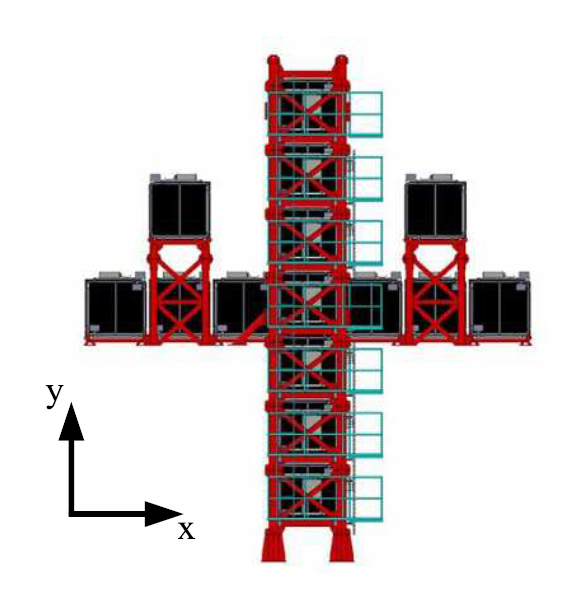
\includegraphics[width=\textwidth]{Figures/ingridcross.png}
    \caption{Schematic of the INGRID cross taken from \cite{t2kcollaborationT2KExperiment2011}.}
    \label{fig:ingridcross}
\end{figure}
\begin{figure}
    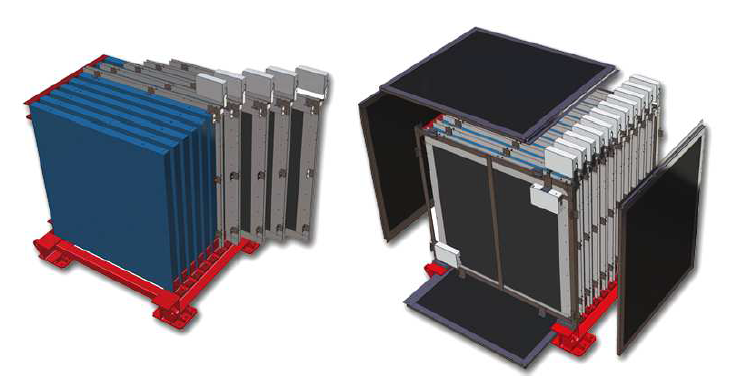
\includegraphics[width=\textwidth]{Figures/ingridmodule.png}
    \caption{Individual INGRID module schematic taken from \cite{t2kcollaborationT2KExperiment2011}.}
    \label{fig:ND280_schematic}
\end{figure}

An additional module, called the proton module was added to measure the muons in combination with protons produced by the neutrino beam in INGRID. This module is used to distinguish the quasi-elastic interaction channel in order to compare it with Monte Carlo simulations of the beamline and neutrino interactions. The Proton Module is made of scintillator planes (no alternating iron plates) and is contained by veto planes. The Proton Module was placed in the centre of the INGRID cross at the intersection of the vertical and horizontal modules. Figure \ref{fig:ingridevent} shows what a standard neutrino event looks like inside the INGRID module. A neutrino enters from the left and after interacting with the scintillator cells (shown in green) produces a tracks (shown in red), with the relative size of each circle corresponding to the observed signal in that cell. The blue cells show the position of the veto scintillators, while the gray planes show the iron plates. 




